\documentclass{article}

\usepackage{graphicx}
\usepackage{tikz}
\usepackage{tikzsymbols}
\usetikzlibrary{calc,patterns,shapes.geometric}
\pagestyle{empty}
\usepackage[margin=0pt]{geometry}
\geometry{papersize={14in,12in}}

\def\centerarc[#1](#2)(#3:#4:#5){\draw[#1] ($(#2)+({#5*cos(#3)},{#5*sin(#3)})$) arc (#3:#4:#5);}

\begin{document}
	\begin{figure}
		\centering
		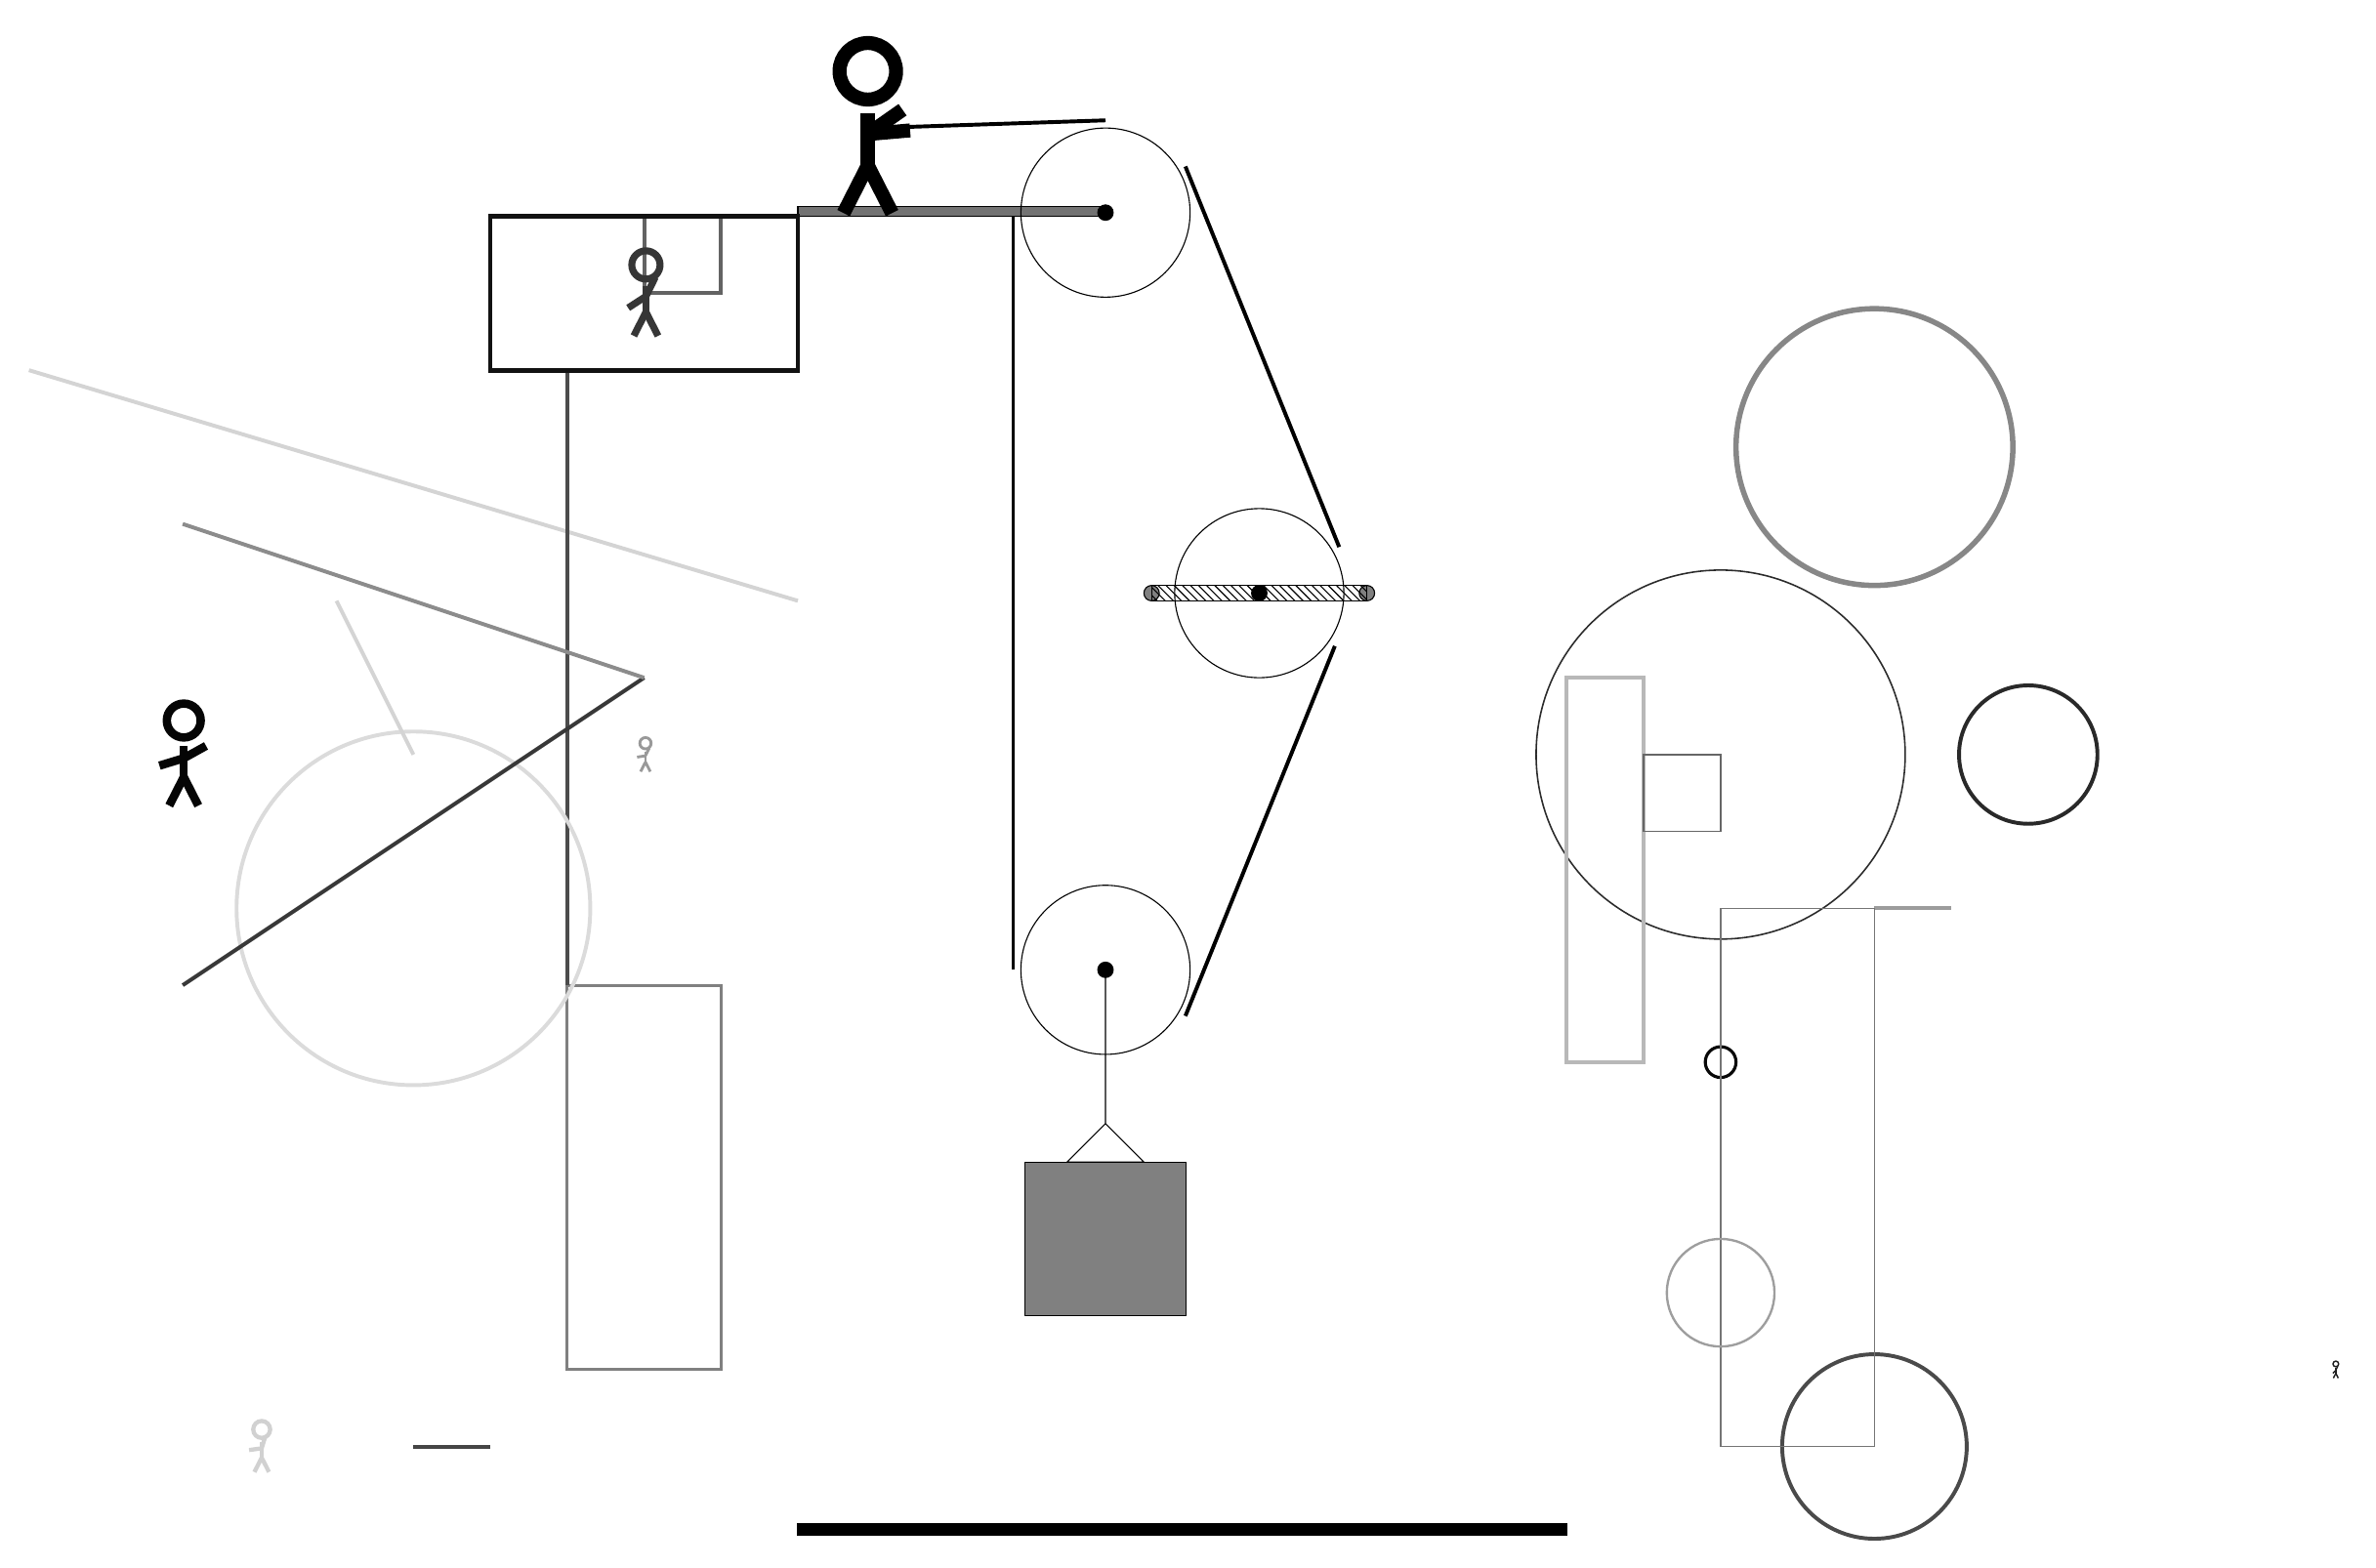
\begin{tikzpicture}
			%%%%% START %%%%%
			
			\draw[fill=black!55] (-2, 14) rectangle (2, 14.125);
			
			\draw (2, 4.2) circle (1.1);
			\draw[fill=black] (2, 4.2) circle (0.1);
			
			\draw (2, 14.05) circle (1.1);
			\draw[fill=black] (2, 14.05) circle (0.1);
			
			\draw[fill=white](4, 9.1) circle (1.1);
			\draw[fill=black] (4, 9.1) circle (0.1);
			\draw[fill=black!50] (2.6, 9.1) circle (0.1);
			\draw[fill=black!50] (5.4, 9.1) circle (0.1);
			\draw[pattern=north west lines, pattern color=black] (2.6, 9.2) rectangle (5.4, 9.0);
			
			\draw (2, 4.2) -- (2, 2.2) -- (1.5, 1.7) -- (2.5, 1.7) -- (2, 2.2);
			\draw[fill=black!50] (0.95, 1.7) rectangle (3.05, -0.3);
			
			\draw[line width=0.4mm, color=black!50] (-3, -1) rectangle (-5, 4);
			
			\draw [line width=0.5mm, color=black!84](14, 7) circle (0.9);
			\node[line width=0.2mm, color=black!98] at (-10, 7) {\Strichmaxerl[6][17][29]};
			\draw[line width=0.5mm, color=black!39](12, 5) -- (13, 5);
			\draw[line width=0.5mm, color=black!17](-2, 9) -- (-12, 12);
			
			\draw[line width=0.5mm, color=black!70](-5, 4) -- (-5, 12);
			
			\draw[line width=0.5mm, color=black!61] (-4, 14) rectangle (-3, 13);
			\draw [line width=0.5mm, color=black!71](12, -2) circle (1.2);
			\node[line width=0.5mm, color=black!79] at (-4, 13) {\Strichmaxerl[5][33][64]};
			
			\draw [line width=0.4mm, color=black!97](10, 3) circle (0.2);
			\draw[line width=0.6mm, color=black!93] (-2, 12) rectangle (-6, 14);
			
			\node[line width=0.2mm, color=black!18] at (-9, -2) {\Strichmaxerl[3][8][73]};
			\draw [line width=0.2mm, color=black!83](10, 7) circle (2.4);
			
			\draw [line width=0.5mm, color=black!14](-7, 5) circle (2.3);
			\draw[line width=0.5mm, color=black!28] (8, 8) rectangle (9, 3);
			\draw[line width=0.2mm, color=black!54] (10, -2) rectangle (12, 5);
			
			\draw[line width=0.5mm, color=black!73](-7, -2) -- (-6, -2);
			
			\draw[line width=0.5mm, color=black!78](-4, 8) -- (-10, 4);
			\draw[line width=0.2mm, color=black!60] (10, 6) rectangle (9, 7);
			
			\draw[line width=0.5mm, color=black!17](-7, 7) -- (-8, 9);
			\draw [line width=0.7mm, color=black!47](12, 11) circle (1.8);
			
			\node[line width=0.6mm, color=black!40] at (-4, 7) {\Strichmaxerl[2][9][64]};
			\draw [line width=0.3mm, color=black!38](10, 0) circle (0.7);
			\node[line width=0.7mm, color=black!88] at (18, -1) {\Strichmaxerl[1][47][64]};
			\draw[line width=0.5mm, color=black!45](-4, 8) -- (-10, 10);
			
			
			\draw[line width=0.5mm] (0.8, 14) -- (0.8, 4.2);
			\centerarc[line width=0.5mm](2, 4.2)(180:330:1.2000000000000002);
			\draw[line width=0.5mm](3.0392, 3.6) -- (4.983, 8.4117);
			\centerarc[line width=0.5mm](4, 9.1)(390:325:1.2000000000000002);
			\draw[line width=0.5mm](5.0392, 9.7) -- (3.0392, 14.65);
			\centerarc[line width=0.5mm](2, 14.05)(30:90:1.2000000000000002);
			\draw[line width=0.5mm](2, 15.25) -- (-1, 15.15);
			
			\node at (-1, 15.15) {\Strichmaxerl[10][-175][35]};
			
			\draw[fill=black] (-2, -3) rectangle (8, -3.15);
			
			%%%%% END %%%%%
		\end{tikzpicture}
	\end{figure}	
\end{document}